\subsection{Vorgehen}
Zur Analyse des Frequenzverhaltens wurde das in Aufgabe~3 hergeleitete (linear) Modell im Frequenzbereich untersucht.
Hierzu wurden in Simulink ein \emph{Linear Input} am Eingangssignal des Lenkwinkels $\delta$ (in Grad) sowie ein
\emph{Linear Output} am Ausgangssignal des Schwimmwinkels $\beta$ (in Grad) gesetzt. Anschlie\ss end wurde das Modell
am Geradeaus-Betriebspunkt ($\delta_0=0$, $\beta_0=0$, $\dot{\Psi}_0=0$) linearisiert und der Frequenzgang
$G(j\omega)=\beta(j\omega)/\delta(j\omega)$ mit Hilfe der Control-System-Analyse (Control System Designer / Linear Analysis)
als Bodediagramm dargestellt. Der in der Aufgabenstellung geforderte Sinuseingang mit der Amplitude $1^\circ$ ist dabei
durch die Normierung des Frequenzgangs abgedeckt: F\"ur ein lineares zeitinvariantes System skaliert die Ausgangsamplitude
im eingeschwungenen Zustand proportional zur Eingangsamplitude, sodass bei $\hat{\delta}=1^\circ$ direkt
$\hat{\beta}(\omega)=|G(j\omega)|\cdot 1^\circ$ gilt.

\begin{figure}[h]
    \centering
    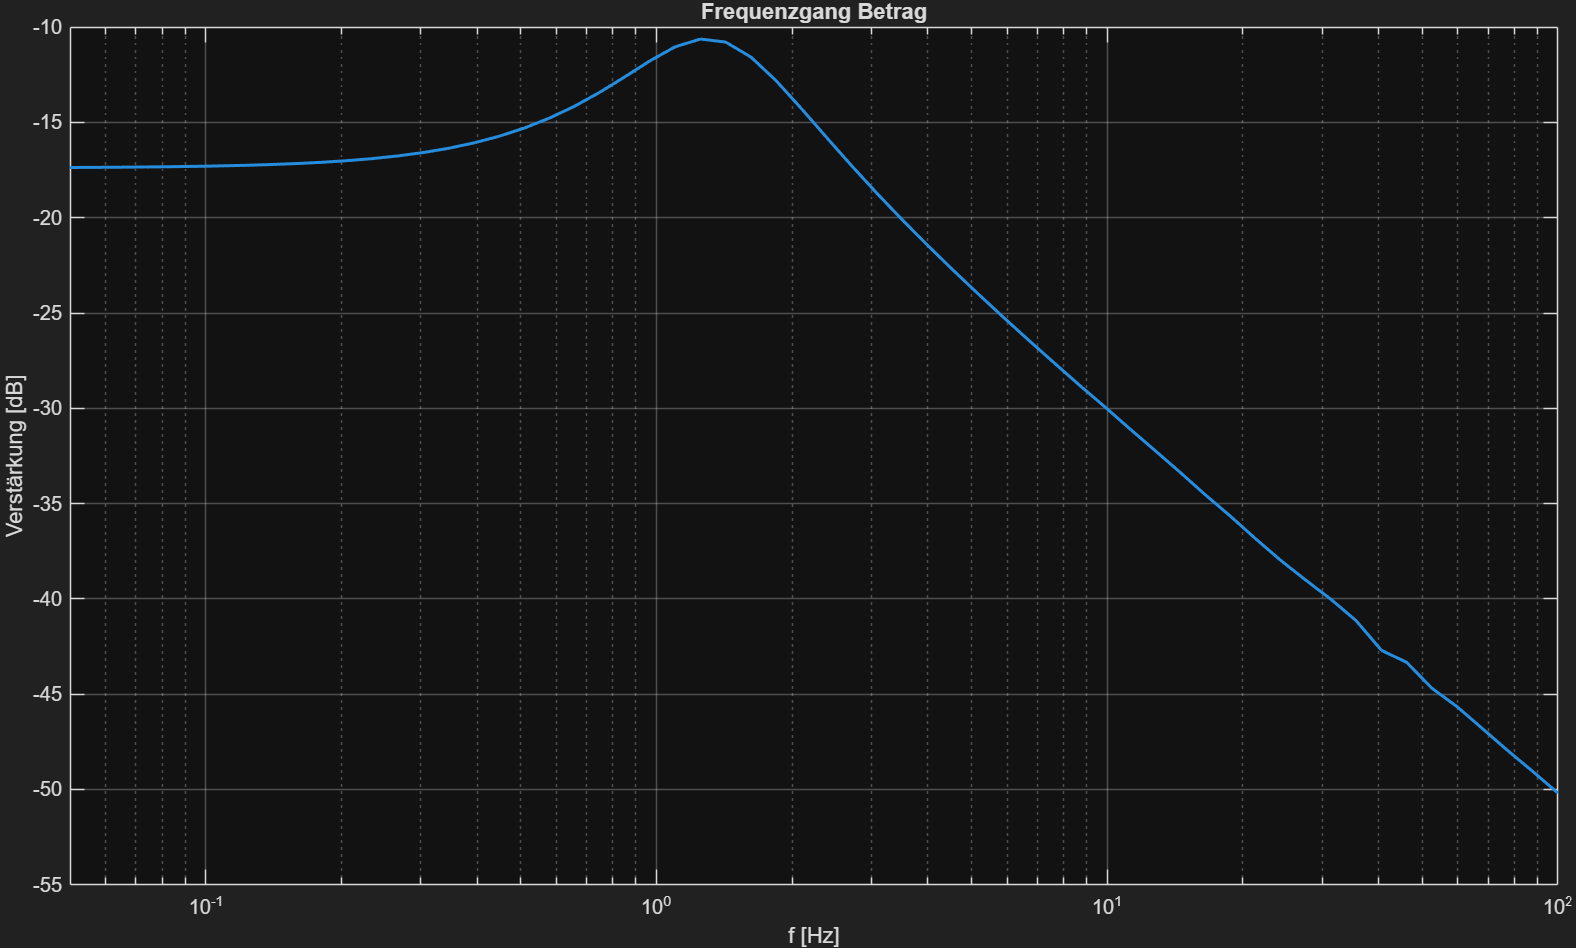
\includegraphics[width=0.95\linewidth]{pictures/Aufgabe4Amplitude.png}
    \caption{Amplitudengang des Schwimmwinkel $\beta$ bei Verwendung des nichtlinearen Einspurmodells bei einem Lenkwinkelsprung auf $1^\circ$.}
    \label{fig:aufgabe4amplitude}
\end{figure}

\begin{figure}[h]
    \centering
    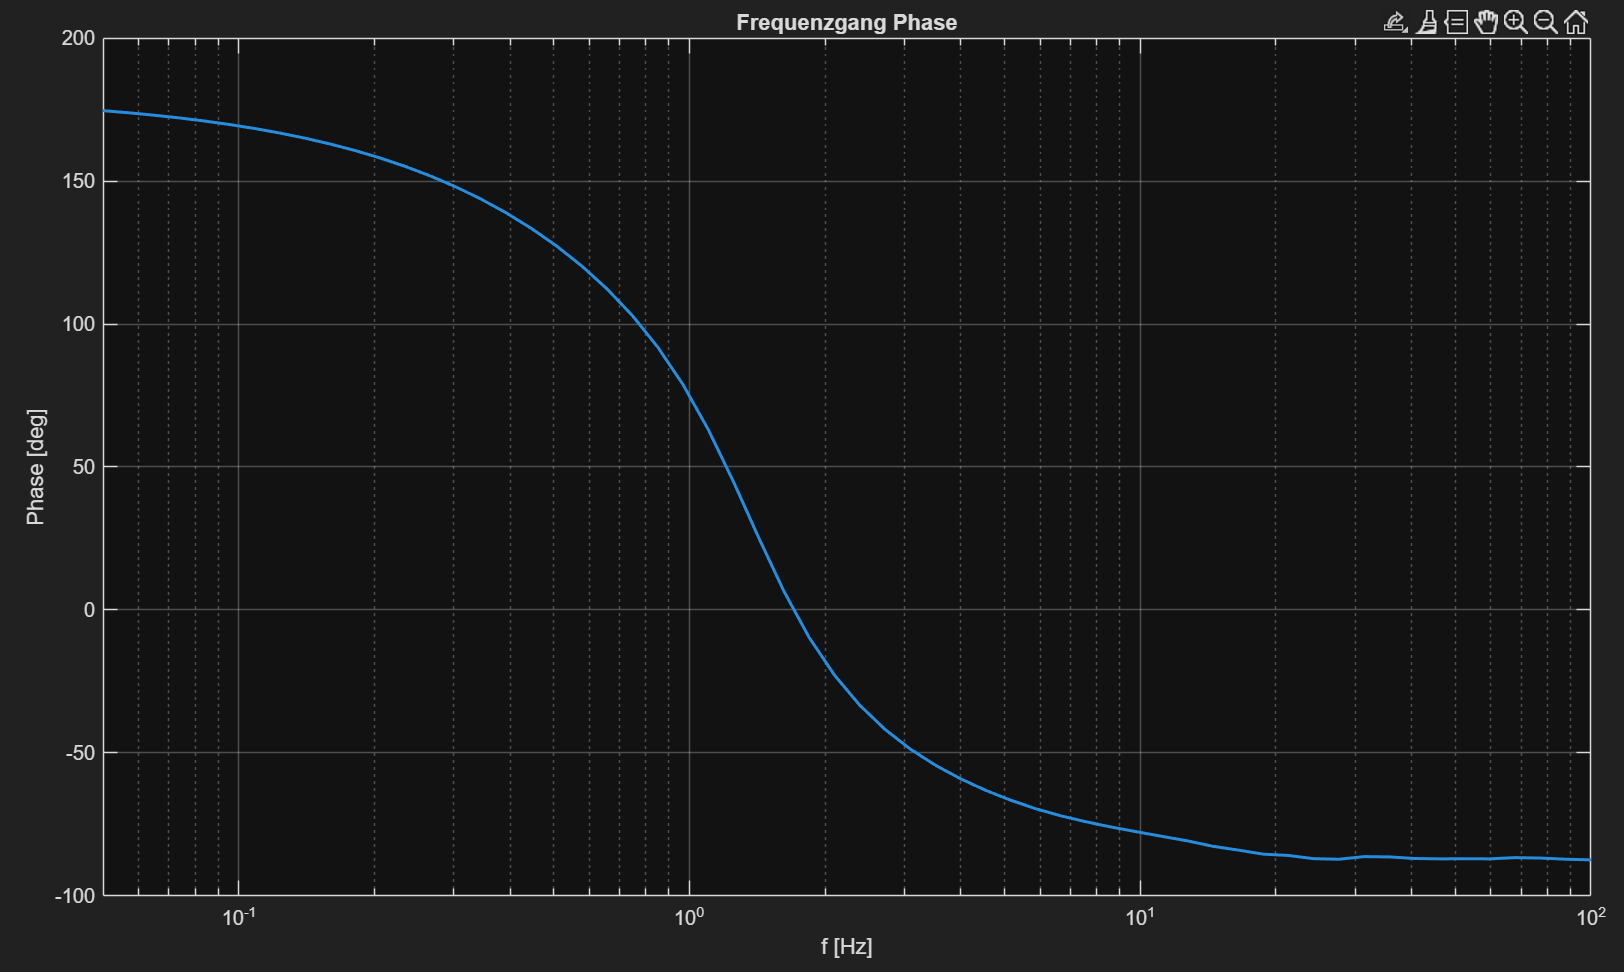
\includegraphics[width=0.95\linewidth]{pictures/Aufgabe4Phase.png}
    \caption{Phasengang des Schwimmwinkel $\beta$ bei Verwendung des nichtlinearen Einspurmodells bei einem Lenkwinkelsprung auf $1^\circ$.}
    \label{fig:aufgabe4phase}
\end{figure}

\subsection{Interpretation}
Die Abbildungen~\ref{fig:aufgabe4amplitude} und~\ref{fig:aufgabe4phase} zeigen den Amplituden- und Phasengang der \"Ubertragungsfunktion von $\delta$ nach $\beta$.
Bei niedrigen Frequenzen ist der Amplitudengang nahezu konstant (ca. $-17\,\mathrm{dB}$), d.\,h.\ langsame Lenkbewegungen
werden vom Fahrzeug quasi-station\"ar nachgebildet und der Schwimmwinkel bleibt im Verh\"altnis zur Lenkanregung klein.
Ein Wert von $-17\,\mathrm{dB}$ entspricht einem Amplitudenverh\"altnis von ungef\"ahr
$|G|\approx 10^{-17/20}\approx 0{,}14$, sodass bei einer Sinusanregung mit $\hat{\delta}=1^\circ$ eine
Schwimmwinkelamplitude von etwa $\hat{\beta}\approx 0{,}14^\circ$ zu erwarten ist.

Im Bereich um $\omega \approx 8$--$10\,\mathrm{rad/s}$ ist eine \"Uberh\"ohung (Peak) erkennbar (ca. $-10\,\mathrm{dB}$).
Dies deutet auf ein unterd\"ampftes Eigenverhalten des Systems hin: Bei Anregung nahe dieser charakteristischen Frequenz
reagiert der Schwimmwinkel \"uberproportional, was im Zeitbereich typischerweise mit \"Uberschwingen bzw. ged\"ampften
Schwingungen einhergeht. Oberhalb dieses Bereichs f\"allt der Amplitudengang stark ab, was einem Tiefpassverhalten entspricht:
Schnelle Lenkanregungen werden aufgrund von Tr\"agheit und Dynamik des Fahrzeugs nur noch stark abgeschw\"acht in $\beta$
abgebildet.

Der Phasengang startet bei niedrigen Frequenzen nahe $180^\circ$ (entspricht einer Vorzeichenumkehr in der gew\"ahlten
Signaldefinition) und dreht im \"Ubergangsbereich stark ab. F\"ur hohe Frequenzen n\"ahert sich die Phase etwa $-90^\circ$,
was ein deutlich verz\"ogertes Folgeverhalten des Schwimmwinkels gegen\"uber der Lenkanregung beschreibt:
Bei schnellen Lenkoszillationen kann das System nicht mehr unmittelbar folgen, sondern reagiert zunehmend phasenverschoben.